\documentclass[11pt]{article}
\usepackage[letterpaper,margin=1in]{geometry}
\usepackage[T1]{fontenc}
\usepackage{lmodern}
\usepackage{microtype}
\usepackage{amsmath,amssymb,amsthm,mathtools}
\usepackage{booktabs,array,longtable}
\usepackage{xcolor}
\usepackage{tikz}
\usetikzlibrary{arrows.meta}
\usepackage[font=small,labelfont=bf]{caption}
\usepackage{hyperref}
\hypersetup{
  colorlinks=true,
  linkcolor=blue!45!black,
  citecolor=blue!45!black,
  urlcolor=blue!45!black,
  pdftitle={Area Moments from a Wallis-Type Geometric Construction},
  pdfauthor={Joshua M. Fitzhugh}
}
\urlstyle{tt}
\setlength{\emergencystretch}{2em}
\numberwithin{equation}{section}
\newtheorem{theorem}{Theorem}[section]
\newtheorem{proposition}[theorem]{Proposition}
\newtheorem{corollary}[theorem]{Corollary}
\theoremstyle{remark}
\newtheorem{remark}[theorem]{Remark}
\newcommand{\R}{\mathbb{R}}
\newcommand{\N}{\mathbb{N}}
\newcommand{\dd}{\,\mathrm{d}}
\newcommand{\Area}{\operatorname{Area}}
\newcommand{\lean}[1]{{\footnotesize\nolinkurl{#1}}}
\newcommand{\proofrevision}{5151013f072b1aaed822bfbc9ee7079fbc7cc2ff}
\newcommand{\prooflink}[2]{%
  \href{https://github.com/speadskater/FitzhughFarnsworth/blob/5151013f072b1aaed822bfbc9ee7079fbc7cc2ff/FitzhughFarnsworth/Wallis/#1.lean}{#2}}

\title{Area Moments from a Wallis-Type\\Geometric Construction}
\author{Joshua M. Fitzhugh}
\date{Draft for review --- November 2026}

\begin{document}
\maketitle

\begin{abstract}
A cyclic construction starts with an $N$-dimensional cube and repeatedly
attaches a rectangular slab of unit volume in each coordinate direction.
For a unit initial cube, Fitzhugh and Farnsworth identified the limiting
longest-to-shortest side ratio with half the area of the planar unit
$N$-circle. We interpret every limiting side ratio in terms of area moments
of that same planar region. Normalization by the shortest side gives the
moments of orders $0,\ldots,N-1$, each multiplied by its order plus two.
A recurrence then recovers every nonnegative integer-order moment.
Allowing arbitrary positive initial cube volume shifts the represented
orders, giving ratios of higher and fractional moments in a fixed
construction dimension. The argument compares classical beta-integral
moment formulas with Gamma-product limits. Its core analytic and geometric
statements are formalized in Lean, including the measured moment integrals
and every intermediate unit-volume attachment.
\end{abstract}

\section{Introduction}
\label{sec:introduction}

Begin with a square of area one. Attach a rectangle of area one across
its right edge, then another of area one across its top edge, and repeat
these two operations. The width-to-height ratio tends to $\pi/2$.
Fitzhugh and Farnsworth~\cite{FitzhughFarnsworth2013} discuss this
construction, attributed there to Myerson, and extend it to rectangles,
boxes, and higher dimensions.

In their $N$-dimensional construction, a unit cube receives unit-volume
slabs cyclically across its coordinate faces. The general limiting
side ratios are expressed as Gamma quotients. The longest-to-shortest
ratio is then identified with half the area enclosed by
\[
  |x|^N+|y|^N=1.
\]
Here $N$ is both the dimension of the box construction and the exponent
of a \emph{planar} curve. The area in this statement is two-dimensional.

The intermediate coordinates suggest a further question: what geometric
quantities do their ratios represent? We show that the normalized sides
give a finite block of weighted area moments of the quarter $N$-disk.
The original half-area identity is its zeroth-order case.
All other ordered side ratios are quotients of entries in this block.
Two extensions follow: a recurrence recovers moments beyond the initial
block, and a change of initial cube volume moves the block to different
moment orders.

Beta and Gamma identities are classical~\cite{DLMF}, and superellipse
moment formulas appear in Jakli\v{c} and Solina~\cite{JaklicSolina2003}.
The unit-cube Gamma ratio already precedes equation~(41)
of~\cite{FitzhughFarnsworth2013}. We give its moment interpretation,
develop the initial-volume parameter, and formally verify the core
arguments while retaining the attachment geometry. This draft does
not establish priority for that interpretation.

\section{Measured moments of the quarter disk}
\label{sec:moments}

For a real exponent $p>0$, let
\begin{equation}
  Q_p=\{(x,y)\in[0,\infty)^2:x^p+y^p\leq 1\}.
  \label{eq:quarter-disk}
\end{equation}
For a real order $r>-1$, define
\begin{equation}
  M_p(r)=\iint_{Q_p}x^r\dd x\dd y,
  \qquad
  W_p(r)=(r+2)M_p(r).
  \label{eq:moments}
\end{equation}
These are moments about the $y$-axis with respect to planar Lebesgue
measure. For $-1<r<0$, the value assigned to $x^r$ on the axis $x=0$
does not affect the integral. Throughout, the coordinate intercepts
of the disk are normalized to one.

\begin{proposition}[Moment evaluation]
\label{prop:moment}
For $p>0$ and $r>-1$, the moment integrand is integrable on $Q_p$,
both $M_p(r)$ and $W_p(r)$ are positive, and
\begin{align}
  M_p(r)
    &=\int_0^1 x^r(1-x^p)^{1/p}\dd x
      =\frac1p B\!\left(\frac{r+1}{p},1+\frac1p\right),
       \label{eq:moment-beta}\\
  W_p(r)
    &=\frac{\Gamma((r+1)/p)\Gamma(1+1/p)}
            {\Gamma((r+2)/p)}.
       \label{eq:weighted-gamma}
\end{align}
\end{proposition}

\begin{proof}
The region $Q_p$ is measurable and lies in $[0,1]^2$.
On this square, $x^r$ is integrable for $r>-1$ because
$\int_0^1 x^r\dd x=1/(r+1)$.
Restricting this integrable function to $Q_p$ gives integrability
of the planar moment, including the orders with an axis singularity.
The vertical section of $Q_p$ at $x\in[0,1]$ is
$[0,(1-x^p)^{1/p}]$, so Fubini's theorem gives the first equality
in~\eqref{eq:moment-beta}.

Substitute $t=x^p$. The result is
\[
  M_p(r)=\frac1p\int_0^1
       t^{(r+1)/p-1}(1-t)^{1/p}\dd t.
\]
Both beta parameters are strictly positive. Euler's beta identity
therefore yields
\[
  M_p(r)=\frac1p\,
    \frac{\Gamma((r+1)/p)\Gamma(1+1/p)}
         {\Gamma(1+(r+2)/p)}.
\]
Using $\Gamma(z+1)=z\Gamma(z)$ and multiplying by $r+2$ gives
\eqref{eq:weighted-gamma}. Positivity follows from positivity of
Gamma at positive real arguments.
\end{proof}

Let $A_p$ be the area of the full disk
$D_p=\{(x,y)\in\R^2:|x|^p+|y|^p\leq1\}$.
The normalizations that will be used below are
\begin{equation}
  W_p(0)=2M_p(0)=\frac{A_p}{2},
  \qquad
  W_p(p-1)=1.
  \label{eq:normalization}
\end{equation}
The first follows by reflection of the quarter disk, and the second
follows directly from~\eqref{eq:weighted-gamma}.
For an integer order $r$, odd \emph{signed} moments over $D_p$ vanish.
The full-disk absolute moment, for any real $r>-1$, is $4M_p(r)$.
Our convention throughout is the first-quadrant moment in
\eqref{eq:moments}, so positive first moments are retained.

\section{The cyclic attachment construction}
\label{sec:construction}

Fix an integer $N\geq2$ and an initial volume $\lambda>0$.
Start with an $N$-cube whose sides are $\lambda^{1/N}$.
In each cycle, update coordinates $0,1,\ldots,N-1$ in this order.
An update attaches a rectangular slab of volume one across the
entire current face perpendicular to the coordinate being updated.
Write $L_i(k;\lambda)$ for side $i$ after $k$ complete cycles.
In particular,
\[
  L_i(0;\lambda)=\lambda^{1/N}.
\]

\begin{figure}[htbp]
\centering
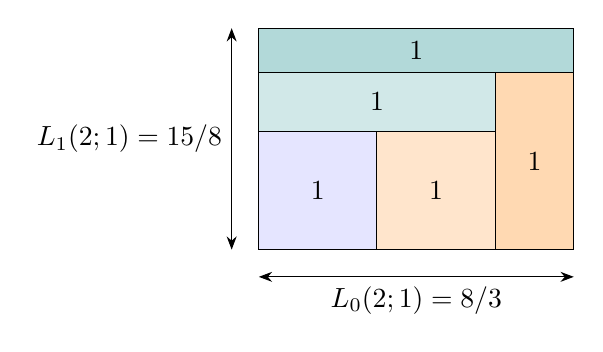
\begin{tikzpicture}[x=1.5cm,y=1.5cm,>=Stealth]
  \fill[blue!10] (0,0) rectangle (1,1);
  \fill[orange!20] (1,0) rectangle (2,1);
  \fill[teal!18] (0,1) rectangle (2,1.5);
  \fill[orange!30] (2,0) rectangle ({8/3},1.5);
  \fill[teal!30] (0,1.5) rectangle ({8/3},{15/8});
  \draw (0,0) rectangle ({8/3},{15/8});
  \draw (1,0)--(1,1) (0,1)--(2,1) (2,0)--(2,1.5)
        (0,1.5)--({8/3},1.5);
  \node at (.5,.5) {$1$};
  \node at (1.5,.5) {$1$};
  \node at (1,1.25) {$1$};
  \node at ({7/3},.75) {$1$};
  \node at ({4/3},{27/16}) {$1$};
  \draw[<->] (0,-.23)--node[below] {$L_0(2;1)=8/3$} ({8/3},-.23);
  \draw[<->] (-.23,0)--node[left] {$L_1(2;1)=15/8$} (-.23,{15/8});
\end{tikzpicture}
\caption{The initial square and four unit-area attachments when $N=2$
and $\lambda=1$. Each marked region has area one. The ratio shown is
the finite value $64/45$; its limit over complete cycles is $\pi/2$.}
\label{fig:attachments}
\end{figure}

\begin{proposition}[Finite geometry]
\label{prop:geometry}
Every side is positive. After $k$ complete cycles and $j$ further
attachments, where $0\leq j\leq N$, the volume is
\begin{equation}
  \lambda+Nk+j.
  \label{eq:intermediate-volume}
\end{equation}
Every attachment changes only its selected coordinate and adds
volume exactly one. The complete-cycle sides satisfy
\begin{equation}
  L_i(k;\lambda)=\lambda^{1/N}
       \prod_{q=0}^{k-1}
          \frac{\lambda+Nq+i+1}{\lambda+Nq+i},
  \qquad 0\leq i<N.
  \label{eq:finite-sides}
\end{equation}
For $k\geq1$, these sides are strictly ordered:
$L_0(k;\lambda)>\cdots>L_{N-1}(k;\lambda)$.
\end{proposition}

\begin{proof}
Suppose the current volume is $V>0$, the selected side has length $a$,
and the product of the other sides is $F>0$. Then $V=aF$.
A slab of volume one has thickness $1/F$, so the new side is
\[
  a+\frac1F=a\left(1+\frac1V\right).
\]
All sides remain positive, the other sides are unchanged, and the
new volume is $V+1$. Induction on individual attachments proves
\eqref{eq:intermediate-volume}.

Immediately before coordinate $i$ is updated in cycle $q$, the
volume is $\lambda+Nq+i$. Its multiplicative update is thus the
factor in~\eqref{eq:finite-sides}; multiplying over the $k$ cycles
proves that formula. For fixed $q$, the positive factor
$1+1/(\lambda+Nq+i)$ is strictly decreasing in $i$.
The initial sides are equal, so their products are strictly ordered
after any positive number of complete cycles.
\end{proof}

\begin{proposition}[Side-ratio limit]
\label{prop:gamma-limit}
For every $i,j\in\{0,\ldots,N-1\}$,
\begin{equation}
  \lim_{k\to\infty}\frac{L_i(k;\lambda)}{L_j(k;\lambda)}
  =
  \frac{\Gamma((\lambda+i)/N)\Gamma((\lambda+j+1)/N)}
       {\Gamma((\lambda+i+1)/N)\Gamma((\lambda+j)/N)}.
  \label{eq:gamma-limit}
\end{equation}
This limit is finite and strictly positive.
\end{proposition}

\begin{proof}
Put $a_i=(\lambda+i)/N$ and $b_i=(\lambda+i+1)/N$.
Both are positive, and $b_i-a_i=1/N$.
The Gamma recurrence gives the finite identity
\[
  \prod_{q=0}^{k-1}\frac{q+b_i}{q+a_i}
  =\frac{\Gamma(k+b_i)\Gamma(a_i)}
         {\Gamma(b_i)\Gamma(k+a_i)}.
\]
Upon taking the ratio for $i$ and $j$, the common initial side
$\lambda^{1/N}$ cancels. The remaining factor depending on $k$ is
\[
  \frac{\Gamma(k+b_i)\Gamma(k+a_j)}
       {\Gamma(k+a_i)\Gamma(k+b_j)}.
\]
It tends to one because $b_i+a_j=a_i+b_j$, by the standard
Gamma-ratio asymptotic
$\Gamma(k+a)/\Gamma(k+b)\sim k^{a-b}$
\cite[Eq.~5.11.12]{DLMF}.
The constant factor is~\eqref{eq:gamma-limit}.
All its Gamma arguments are positive.
\end{proof}

\section{The moment interpretation}
\label{sec:correspondence}

\begin{theorem}[Construction--moment correspondence]
\label{thm:correspondence}
For $N\geq2$, $\lambda>0$, and $0\leq i,j<N$,
\begin{equation}
  \boxed{\displaystyle
  \lim_{k\to\infty}\frac{L_i(k;\lambda)}{L_j(k;\lambda)}
    =\frac{W_N(\lambda+i-1)}{W_N(\lambda+j-1)}.}
  \label{eq:correspondence}
\end{equation}
The moment orders on the right are greater than $-1$.
\end{theorem}

\begin{proof}
Since $\lambda>0$ and $i,j\geq0$, both orders are in the range
of Proposition~\ref{prop:moment}. Equation~\eqref{eq:weighted-gamma}
gives
\[
  W_N(\lambda+i-1)
    =\frac{\Gamma((\lambda+i)/N)\Gamma(1+1/N)}
            {\Gamma((\lambda+i+1)/N)}.
\]
The quotient of this expression and its counterpart for $j$
cancels the common positive factor $\Gamma(1+1/N)$.
The result is~\eqref{eq:gamma-limit}.
\end{proof}

Write $d_i(k)=L_i(k;1)$ for the original unit-cube construction.
Its shortest coordinate after a positive number of cycles is
$d_{N-1}(k)$.

\begin{corollary}[Normalized sides]
\label{cor:unit}
For $0\leq i<N$,
\begin{equation}
  \lim_{k\to\infty}\frac{d_i(k)}{d_{N-1}(k)}
     =W_N(i)=(i+2)M_N(i).
  \label{eq:unit-moments}
\end{equation}
Consequently, the coordinatewise limiting normalized side vector is
\begin{equation}
  \bigl(2M_N(0),\,3M_N(1),\,\ldots,\,NM_N(N-2),\,1\bigr).
  \label{eq:side-vector}
\end{equation}
\end{corollary}

\begin{proof}
Use $\lambda=1$ and $j=N-1$ in
Theorem~\ref{thm:correspondence}, and then apply
$W_N(N-1)=1$ from~\eqref{eq:normalization}.
\end{proof}

For $i=0$, equation~\eqref{eq:unit-moments} reads
\[
  \lim_{k\to\infty}\frac{d_0(k)}{d_{N-1}(k)}
     =2M_N(0)=\frac{A_N}{2}.
\]
This is equation~(41) of~\cite{FitzhughFarnsworth2013}.
Thus the half-area interpretation sits inside a sequence of
first-quadrant area moments.

For any two coordinates,
\begin{equation}
  \lim_{k\to\infty}\frac{d_i(k)}{d_j(k)}
    =\frac{(i+2)M_N(i)}{(j+2)M_N(j)}.
  \label{eq:all-pairs}
\end{equation}
Reversing the ordered pair takes the reciprocal, since all moments
are positive. Ratios to the shortest side give individual weighted
moments; arbitrary pairs generally give quotients of such moments.
These statements concern limits. They do not identify a finite
stage of the construction with the limiting moment values.

\section{Recovery of higher-order moments}
\label{sec:recurrence}

\begin{proposition}[Moment recurrence]
\label{prop:recurrence}
For any $p>0$ and $r>-1$,
\begin{align}
  M_p(r+p)&=\frac{r+1}{r+p+2}M_p(r), \label{eq:raw-recurrence}\\
  W_p(r+p)&=\frac{r+1}{r+2}W_p(r).   \label{eq:weighted-recurrence}
\end{align}
For every nonnegative integer $q$,
\begin{equation}
  W_p(r+qp)=W_p(r)
       \prod_{h=0}^{q-1}\frac{r+hp+1}{r+hp+2}.
  \label{eq:ladder}
\end{equation}
An empty product is one.
\end{proposition}

\begin{proof}
Replacing $r$ by $r+p$ in~\eqref{eq:weighted-gamma} increases both
Gamma arguments containing $r$ by one. Applying the Gamma recurrence
to numerator and denominator gives the multiplier $(r+1)/(r+2)$.
Substituting $W_p(r)=(r+2)M_p(r)$ gives~\eqref{eq:raw-recurrence}.
Iteration proves~\eqref{eq:ladder}. Every intermediate order is greater
than $-1$, and every displayed denominator is positive.
\end{proof}

\begin{corollary}[Every integer order from the original sides]
\label{cor:recovery}
Fix $N\geq2$ and a nonnegative integer $m$.
Write $m=a+qN$ with $0\leq a<N$. Then
\begin{equation}
  M_N(m)=
   \lim_{k\to\infty}
   \left[
     \frac{d_a(k)}{d_{N-1}(k)}
     \frac{1}{m+2}
     \prod_{h=0}^{q-1}\frac{a+hN+1}{a+hN+2}
   \right].
   \label{eq:all-orders}
\end{equation}
\end{corollary}

\begin{proof}
Apply~\eqref{eq:ladder} with $p=N$ and $r=a$.
Corollary~\ref{cor:unit} supplies $W_N(a)$ as the limit of an
actual coordinate ratio. Multiplication by the displayed constant
and division by $m+2>0$ give~\eqref{eq:all-orders}.
\end{proof}

There are only $N-1$ potentially nontrivial normalized side values;
the last is one. The recurrence determines the later moments from
these values and the known normalization. Equation~\eqref{eq:all-orders}
does not introduce additional geometric coordinates, and it does not
assert arithmetic independence of the initial moment values.

\section{Examples and geometric meaning}
\label{sec:examples}

\subsection{The circle and moments beyond dimension two}

For $N=2$,
\[
  W_2(0)=\frac{\pi}{2},\qquad W_2(1)=1.
\]
The recurrence generates the even and odd orders separately:
\[
  W_2(2)=\frac{\pi}{4},\qquad
  W_2(3)=\frac23,\qquad
  W_2(4)=\frac{3\pi}{16}.
\]
Hence
\[
  M_2(0)=\frac{\pi}{4},\quad M_2(1)=\frac13,\quad
  M_2(2)=\frac{\pi}{16},\quad M_2(3)=\frac{2}{15},\quad
  M_2(4)=\frac{\pi}{32}.
\]
The second area moment of the full unit disk about its $y$-axis
is $4M_2(2)=\pi/4$. Thus it is one half of the original
limiting rectangle ratio. A separate coordinate is unnecessary
once the recurrence is known.

\subsection{The quartic disk}

For $N=4$, the limiting normalized sides are
\begin{equation}
  \bigl(W_4(0),W_4(1),W_4(2),W_4(3)\bigr)
  =
  \left(
    \frac{\Gamma(1/4)^2}{4\sqrt{\pi}},
    \frac{\sqrt{\pi}\,\Gamma(1/4)}{4\Gamma(3/4)},
    \frac{\pi}{2\sqrt{2}},
    1
  \right).
  \label{eq:quartic}
\end{equation}
The special-function reductions use
$\Gamma(1/2)=\sqrt{\pi}$ and
$\Gamma(1/4)\Gamma(3/4)=\pi\sqrt{2}$.
The decimal values below are numerical illustrations.

\begin{center}
\begin{tabular}{@{}clrr@{}}
\toprule
Coordinate $i$ & Limit $d_i/d_3$ & Weighted moment & Approximation\\
\midrule
0 & $W_4(0)$ & $2M_4(0)$ & $1.85407468$\\
1 & $W_4(1)$ & $3M_4(1)$ & $1.31102878$\\
2 & $W_4(2)$ & $4M_4(2)$ & $1.11072073$\\
3 & $1$      & $5M_4(3)$ & $1.00000000$\\
\bottomrule
\end{tabular}
\end{center}

\begin{figure}[htbp]
\centering
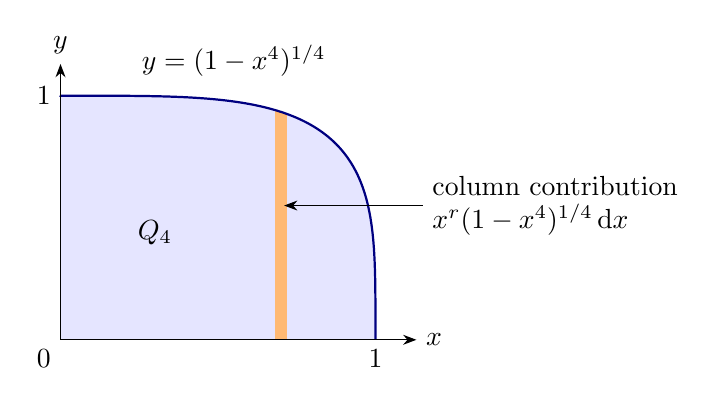
\begin{tikzpicture}[x=4cm,y=3.1cm,>=Stealth]
  \fill[blue!10] (0,0)--(1,0)
    --plot[domain=0:90,samples=120]
      ({sqrt(max(0,cos(\x)))},{sqrt(max(0,sin(\x)))})--(0,1)--cycle;
  \begin{scope}
    \clip (0,0)--(1,0)
      --plot[domain=0:90,samples=120]
        ({sqrt(max(0,cos(\x)))},{sqrt(max(0,sin(\x)))})--(0,1)--cycle;
    \fill[orange!55] (.68,0) rectangle (.72,1.1);
  \end{scope}
  \draw[thick,blue!50!black,domain=0:90,samples=120]
    (1,0)--plot ({sqrt(max(0,cos(\x)))},{sqrt(max(0,sin(\x)))})--(0,1);
  \draw[->] (0,0)--(1.13,0) node[right] {$x$};
  \draw[->] (0,0)--(0,1.13) node[above] {$y$};
  \node[below left] at (0,0) {$0$};
  \node[below] at (1,0) {$1$};
  \node[left] at (0,1) {$1$};
  \node at (.30,.44) {$Q_4$};
  \node[above] at (.55,1.04) {$y=(1-x^4)^{1/4}$};
  \draw[->] (1.15,.55)--(.71,.55);
  \node[right,align=left] at (1.15,.55)
    {column contribution\\$x^r(1-x^4)^{1/4}\dd x$};
\end{tikzpicture}
\caption{The moment is the integral of vertical-column area weighted by
$x^r$. This is a planar region, although its weighted moments describe
side ratios of the four-dimensional construction.}
\label{fig:moment}
\end{figure}

Let $A_Q=M_4(0)$, let $\bar{x}=M_4(1)/M_4(0)$ be the
quarter-disk centroid coordinate, and let
$k_y^2=M_4(2)/M_4(0)$ be its squared radius of gyration about
the coordinate $y$-axis. Equation~\eqref{eq:all-pairs} gives
\[
  \lim_{k\to\infty}\frac{d_0(k)}{d_1(k)}
       =\frac{2}{3\bar{x}}=\sqrt{2},
  \qquad
  \lim_{k\to\infty}\frac{d_2(k)}{d_0(k)}=2k_y^2.
\]
These ratios describe geometric combinations of moments; neither
should be described as a new, independent raw moment.
The next four weighted moments are
\[
  W_4(4)=\tfrac12 W_4(0),\quad
  W_4(5)=\tfrac23 W_4(1),\quad
  W_4(6)=\tfrac34 W_4(2),\quad
  W_4(7)=\tfrac45.
\]

\section{Selecting moment orders through the initial volume}
\label{sec:volume}

For a fixed construction dimension $N$, the initial volume $\lambda$
selects the consecutive orders
\begin{equation}
  \lambda-1,\ \lambda,\ \ldots,\ \lambda+N-2.
  \label{eq:orders}
\end{equation}
Theorem~\ref{thm:correspondence} gives the ratios between their
weighted moments.

\begin{corollary}[Arbitrary real starting order]
\label{cor:fractional}
For $N\geq2$ and any real $r>-1$, start with cube volume
$\lambda=r+1$. Then
\begin{equation}
  \lim_{k\to\infty}
    \frac{L_0(k;r+1)}{L_1(k;r+1)}
       =\frac{W_N(r)}{W_N(r+1)}.
  \label{eq:adjacent}
\end{equation}
\end{corollary}

\begin{proof}
The initial volume is positive. Apply
Theorem~\ref{thm:correspondence} with $i=0$ and $j=1$.
\end{proof}

For integer orders, one can also compare successive constructions
with initial volumes
\[
  1,\ N,\ 2N-1,\ 3N-2,\ldots.
\]
Each new block in~\eqref{eq:orders} shares its first order with
the last order of the preceding block. A known moment at that
shared order fixes the scale of the new block: if the starting
order is $a$, multiply the limiting ratio $L_i/L_0$ by $W_N(a)$.
The first shared value is $W_N(N-1)=1$.
This gives a geometric way to extend the displayed orders while
keeping $N$ fixed.

For example, in dimension two the initial areas $1,2,3,4$ give
the limiting first-to-second side ratios
\[
  \frac{W_2(0)}{W_2(1)}=\frac{\pi}{2},\qquad
  \frac{W_2(1)}{W_2(2)}=\frac4\pi,\qquad
  \frac{W_2(2)}{W_2(3)}=\frac{3\pi}{8},\qquad
  \frac{W_2(3)}{W_2(4)}=\frac{32}{9\pi}.
\]
For noninteger $\lambda$, the same process represents fractional
orders. It gives their \emph{ratios}; an absolute moment value
requires a known normalization, for example
Proposition~\ref{prop:moment}. The finite collection of integer
seed moments alone is not a claim to determine all real-order
moments by the integer-step recurrence.

\section{Formal verification and reproducibility}
\label{sec:formalization}

The core results are formalized in Lean~4~\cite{Lean4}, using
mathlib~\cite{Mathlib}. The definitions retain the objects in the
proofs above. In particular, \lean{quarterMoment} is a set integral
against planar Lebesgue measure, not a definition by its Gamma
value. Its equality to the one-dimensional integral is proved
using Fubini and explicit vertical sections.
For the generalized construction, each coordinate state is a
function on \lean{Fin N}. Positive side lengths, intermediate
volume, and the volume-one attachment equation are proved
before the moment interpretation is applied.

Table~\ref{tab:lean} records the principal entry points. All names
are in the namespace \lean{FitzhughFarnsworth.Wallis}; the prefixes
\lean{Hypercube} and \lean{ShiftedHypercube} distinguish the original
and arbitrary-starting-volume constructions.

\begingroup
\small
\renewcommand{\arraystretch}{1.15}
\begin{longtable}{@{}>{\raggedright\arraybackslash}p{.29\textwidth}%
  >{\raggedright\arraybackslash}p{.67\textwidth}@{}}
\caption{Correspondence between the mathematical statements and Lean
declarations. Module links refer to the fixed proof revision.}
\label{tab:lean}\\
\toprule
Statement & Module and principal declarations\\
\midrule
\endfirsthead
\toprule
Statement & Module and principal declarations\\
\midrule
\endhead
\bottomrule
\endfoot
Proposition~\ref{prop:moment}, integrability and substitution &
  \prooflink{MomentIntegrals}{MomentIntegrals}:
  \lean{moment_intervalIntegrable},
  \lean{momentIntegral_substitution},
  \lean{momentIntegral_eq_gamma}\\
Proposition~\ref{prop:moment}, measured moments &
  \prooflink{Moments}{Moments}:
  \lean{integrableOn_quarterMoment},
  \lean{quarterMoment_eq_integral},
  \lean{quarterMoment_eq_gamma},
  \lean{weightedMoment_eq_gamma},
  \lean{weightedMoment_pos}\\
Proposition~\ref{prop:geometry}, individual attachments &
  \prooflink{ShiftedHypercube}{ShiftedHypercube}:
  \lean{side_pos}, \lean{volume_partial},
  \lean{attachment_volume}, \lean{partial_step_other},
  \lean{dimensions_strictAnti}\\
Proposition~\ref{prop:gamma-limit} &
  \prooflink{ShiftedHypercube}{ShiftedHypercube}:
  \lean{ratio_eq_linear_prod}, \lean{ratio_tendsto}\\
Theorem~\ref{thm:correspondence} &
  \prooflink{MomentRatios}{MomentRatios}:
  \lean{ShiftedHypercube.ratio_tendsto_moments}\\
Corollary~\ref{cor:unit} and equation~\eqref{eq:all-pairs} &
  \prooflink{MomentRatios}{MomentRatios}:
  \lean{Hypercube.normalized_side_tendsto},
  \lean{Hypercube.ratio_tendsto_moments}\\
Proposition~\ref{prop:recurrence} &
  \prooflink{Moments}{Moments}:
  \lean{quarterMoment_add_exponent},
  \lean{weightedMoment_add_exponent},
  \lean{weightedMoment_add_nat_mul}\\
Corollary~\ref{cor:recovery} &
  \prooflink{Moments}{Moments}:
  \lean{weightedMoment_nat_eq};
  \prooflink{MomentRatios}{MomentRatios}:
  \lean{Hypercube.scaled_ratio_tendsto_quarterMoment}\\
Corollary~\ref{cor:fractional} &
  \prooflink{MomentRatios}{MomentRatios}:
  \lean{ShiftedHypercube.adjacent_moment_ratio_tendsto}\\
Exact unit-volume starting case &
  \prooflink{ShiftedHypercube}{ShiftedHypercube}:
  \lean{side_one}, \lean{dimensions_one},
  \lean{partialDimensions_one}\\
\end{longtable}
\endgroup

The moment and recurrence results hold for every real $p>0$ and
$r>-1$, including nonconvex $Q_p$ when $0<p<1$.
The construction results hold for every integer $N>0$; this paper
uses $N\geq2$ to discuss distinct side coordinates.
Its coordinate labels are zero-based, so coordinate $i$ corresponds
to coordinate $i+1$ in Section~5.3 of~\cite{FitzhughFarnsworth2013}.

The proof revision is
\begin{center}
\small\texttt{\proofrevision}.
\end{center}
It uses Lean \lean{v4.36.0-rc2} and mathlib revision
\begin{center}
\small\texttt{cbe1882f5b62496bdfc6bbe540a2b3f2db852440}.
\end{center}
The source is available in the
\href{https://github.com/speadskater/FitzhughFarnsworth}{FitzhughFarnsworth repository}.
A full build and an audit of all 1,706 project declarations pass;
the audit includes private declarations and permits only the standard
axioms \lean{propext}, \lean{Classical.choice}, and \lean{Quot.sound}.
There are no admitted proofs or project-specific mathematical axioms.
The declaration checks run 15 environment linters.

Table~\ref{tab:lean} identifies the formal core. The decimal values
and special-value simplifications in Section~\ref{sec:examples},
the reflection comments, and the comparison of overlapping blocks
are expository consequences rather than additional independently
certified Lean declarations. Human review is still needed to assess
the exposition, its correspondence with the formal statements, and
the contribution relative to the literature.

\begin{samepage}
\subsection*{AI-assistance disclosure}

OpenAI ChatGPT and Codex assisted with mathematical exploration,
Lean proof development, and preparation of this manuscript.
The draft has not undergone independent human mathematical review.
The Lean verification and the preliminary literature search do not
constitute a claim of publication priority.

\end{samepage}

\begingroup
\raggedright
\bibliographystyle{plain}
\bibliography{references}
\endgroup

\end{document}
